\documentclass[11pt]{article}
\usepackage{fullpage}
\usepackage{natbib}
\usepackage{url}
\usepackage{graphicx}

%opening
\title{Computational analysis of the Etch-A-Sketch task:\\ a commentary on Annand et al. (2020)}
\author{}

\begin{document}

\maketitle

%\begin{abstract}
%\end{abstract}

\citet{Annand2020} presented participants with a novel task setup. Their apparatus consists of a stylus on a computer screen controlled by two rotary dials. One dial controlled the $X$-direction of the stylus while the other dial was used to control the $Y$-direction of the stylus. In this, the setup is reminiscent of \textit{Etch-A-Sketch}, the famous mechanical drawing device \citep{EtchASketch}. Using this apparatus, participants were instructed to trace out a circle on the computer screen by following a target indicator. The indicator moved along a circular path with a period of either $\sim$5 seconds or  $\sim$2.5 seconds.

Participants' performance in following the target indicator was evaluated as a function of the trial number. With increased practice, participants' errors decreased. More interestingly, \citet{Annand2020} had individual participants or dyads performing the task. When individuals performed the task, participants controlled both dials. Dyads controlled one dial each.

\citet{Annand2020} present several hypotheses about how the (relative) performance of dyads and individuals would increase with practice. Their predictions suggest that \citet{Annand2020} have not performed a computational assessment of the task preventing them from appreciating the strategies available to participants. As \citet{Annand2020} conclude that their setup can be \textit{[used] to probe many different hypotheses of interlimb coordination and motor learning}, we think it is essential to provide a computational analysis. This would allow researchers using this paradigm to appreciate which conclusions it allows to draw (and which deductions are erroneous).

\citet{Annand2020} assumed that the task requires individuals to reconfigure the pre-existing \textit{intrinsic coordination dynamics} between limbs. The authors assume that, for an individual, moving both arms (or hands) in-phase (or anti-phase) is easier than maintaining the 90 degrees offset in arm movement required by the task. Indeed, to draw a circle on the screen, the rotation of one dial should lag (or lead) the other one by 90 degrees. In contrast, dyads should not experience this problem and are hypothesized to perform better initially. Thus far, we agree with the interpretation of the task.

However, \citet{Annand2020} make an error when they state that individuals potentially could outperform dyads by reconfiguring the coupling between limbs to maintain a 90-degree offset. With this assertion, \citet{Annand2020} assume that individuals could achieve better performance than dyads by (learning to) fix the movement of the arms with a 90 degree offset. Indeed they state that \textit{[G]reater coupling strength [could give] rise to stronger intrinsic coordination dynamics. [O]ver the course of learning, [this could] be harnessed to achieve more rapid stabilization (and hence better performance) of the new [90-degree] coordination pattern.}

This assertion shows that \citet{Annand2020} do not appreciate that the task they present to participants consists of two independent tasks. Indeed, there exists a strategy under which the task can be performed perfectly (zero error) that does not require any coupling or coordination between the limbs. Therefore, there is no benefit from reconfiguring the coupling between limbs. 

Therefore, the task presented by \citet{Annand2020} can not be used to assess how people reconfigure the coupling between limbs. Indeed, any increase in performance can be either attributed to a change in coupling (from 0/180 degrees to 90 degrees), or, alternatively, to an abolition of coupling. The task does not allow distinguishing between these two alternatives. Therefore, at best, the task can be used to conclude that \textit{something} changes in the coupling of limbs. 

In this letter, we present evidence to support our assessment of the task presented by \citet{Annand2020} in the following form. First, we present a simple computational model showing that the task consists of two decoupled sub-tasks. Second, we reanalysis the data presented by \citet{Annand2020} showing that participants did indeed learn to decouple their limbs. Third, we present a Monte Carlo simulation to show that coupling the limbs with an offset of 90 degrees could, in principle, reduce the error but the conditions for this to arise are very limited.


\section{Computational analysis}

In this section, we analyze the task presented by \citet{Annand2020} to show that it consists of two independent tasks. There are multiple ways in which this could be demonstrated. However, as \citet{Annand2020} focus on learning, we show that an agent can perfectly solve the task by learning to decouple both controls.


We use the neural network depicted in figure \ref{fig:neuralnetwork} as a learning agent. The network consists of two input neurons and two output neurons. The neurons have hyperbolic tangent activation functions. The network is trained to produce sinoid output signals $T_1$ and $T_2$ at output neurons $O_1$ and $O_2$, with $T_2$ shifted by 90 degrees with respect to $T_1$.

\begin{figure*}
	\centering
	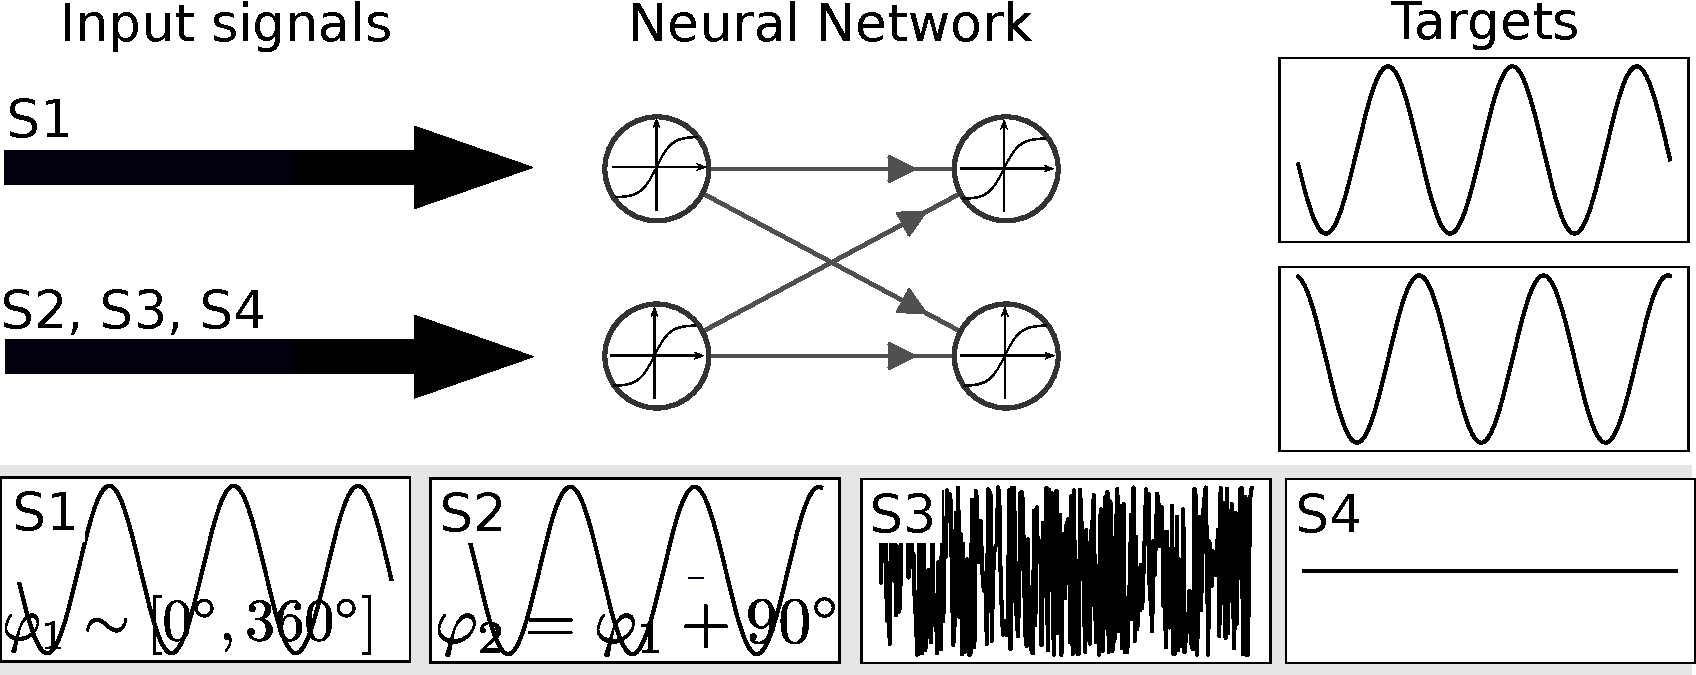
\includegraphics[width=1\linewidth]{neural_network}
	\caption{eqeqeqqqweqeweq}
	\label{fig:neuralnetwork}
\end{figure*}

We varied the input to neuron $I_2$ to demonstrate that the  task of \citet{Annand2020} consists of two independent subtasks. We trained the neural network to produce the desired output in response to various input signals ($S_1$, $S_2$, $S_3$, and $S4$, figure \ref{fig:neuralnetwork} ). The input signal for neuron $I_1$ is fixed to signal $S_1$, a sinoid wave with a length of 3 periods. Its phase was randomized for each training iteration, i.e., $\varphi_1 \sim [0^\circ, 360^\circ]$.



Signal $S_2$ was a sinoid with phase  $ \varphi_2 = \varphi_1 + 90^\circ$. Therefore, when presenting signals $S_1$ and $S_2$ to the neural network as input, we model the task as presented to participants by \citet{Annand2020}: a circular input (target location) has to be converted to a circular output (stylus location). 

Converting $S_1$ and $S_2$ to $T_1$ and $T_2$ is a trivial learning task. After training, the network performs almost perfectly (figure \ref{fig:neuralnetwork0}). The generated output signals are identical to the desired targets. Crucially, we can assess the matrix of network weights to learn how the network solves this task. Inspecting the learned weights shows that the network learned the task decoupling both inputs: the connection between $I_1$ ($I_2$) and $O_2$ ($O_1$) are set to zero.


\begin{figure*}
	\centering
	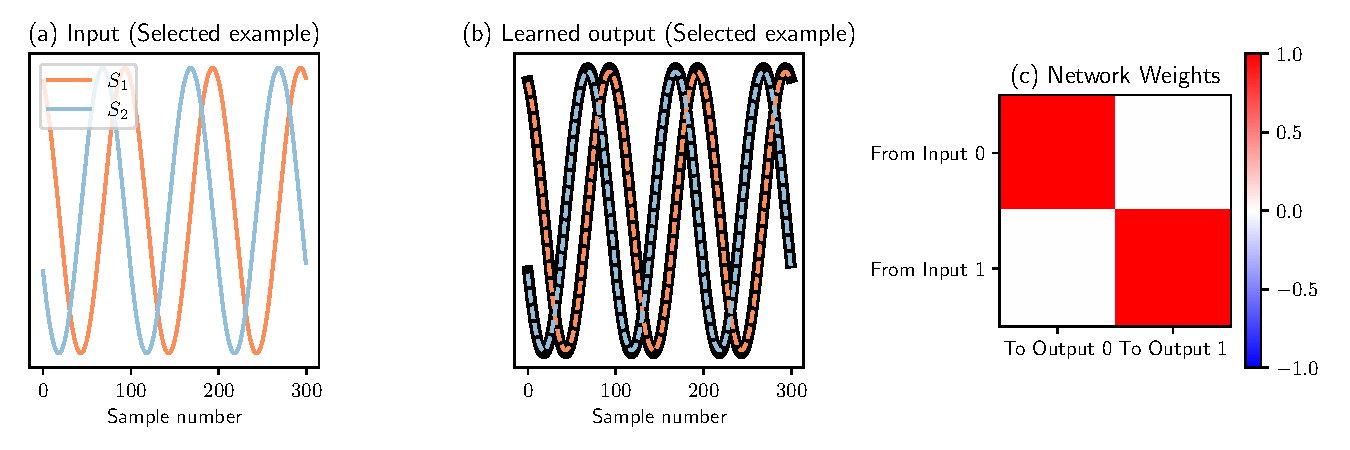
\includegraphics[width=1\linewidth]{neural_network_0}
	\caption{The network depicted in figure \ref{fig:neuralnetwork} was trained to produce sinoid output signals $T_1$ and $T_2$ as response to input signals $S_1$ and $S_2$. (a) An example of input signals $S_1$ and $S_2$. The phase $\varphi_1$ of $S_1$ was varied throughout training while the phase of $S_1$ was offset by $90^\circ$. (b) The output overlaid onto $T_1$ and $T_2$. (c) The resulting network weights.}
	\label{fig:neuralnetwork0}
\end{figure*}

The results depicted in figure \ref{fig:neuralnetwork0} are sufficient to demonstrate that the task presented by \citet{Annand2020} consists of two tasks that can be solved independently. However, to drive this point home, we trained the neural network with two additional inputs to $I_2$: $S_3$ and $S_4$. 

Using $S_3$, we present a random signal to input neuron $I_2$. This prevents the network from learning to generate $T_2$. However, despite the noisy input on neuron $I_2$, the network can still generate the desired output on neuron $O_1$ (figure \ref{fig:neuralnetwork1}). This shows that the network (and, therefore, participants) cansolve half of the task perfectly (e.g, controlling the $Y$-position of the stylus), irrespective of whether they succeed in the other half of the task (e.g., controlling the $Y$-position of the stylus). The network simply learns to ignore the input from $I_2$ (weights originating from this neuron are set to zero). The same conclusion can be drawn from figure  \ref{fig:neuralnetwork2}, using $S_4$ as input for $I_2$. Input signal $S_4$ is clamped to zero but does not interfere with learning to produce $T_2$ in response to $S_1$.

\begin{figure*}
	\centering
	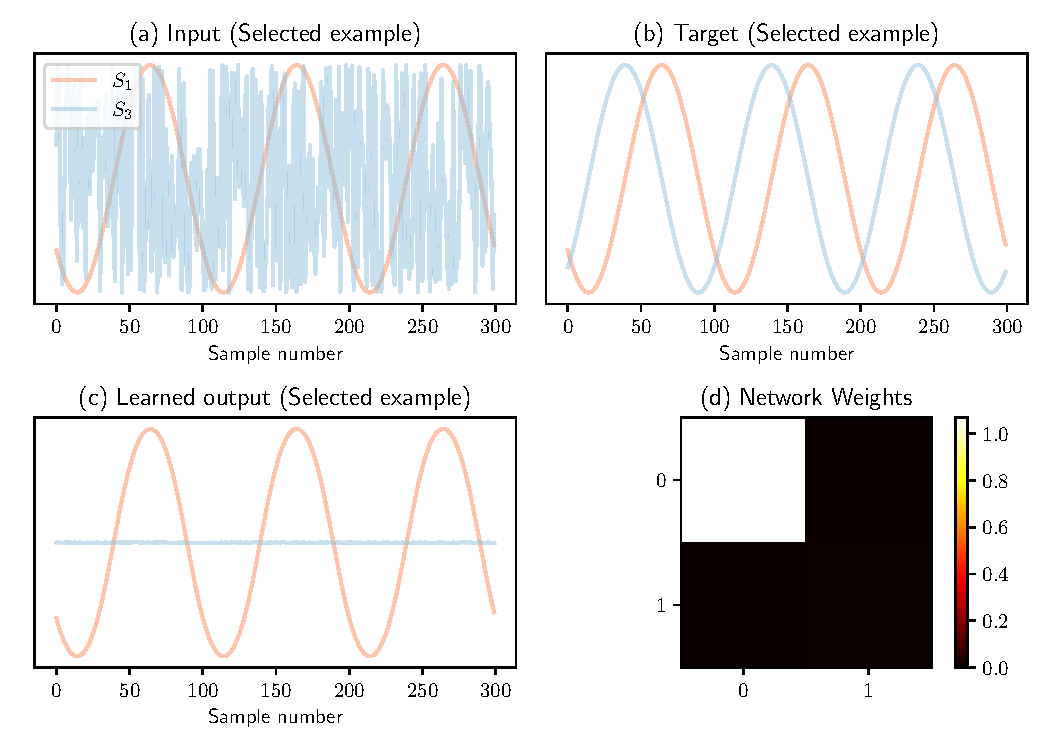
\includegraphics[width=1\linewidth]{neural_network_1}
	\caption{Similar to figure \ref{fig:neuralnetwork0} but for input signal $S_3$ applied to input $I_2$.}
	\label{fig:neuralnetwork1}
\end{figure*}



\begin{figure*}
  	\centering
  	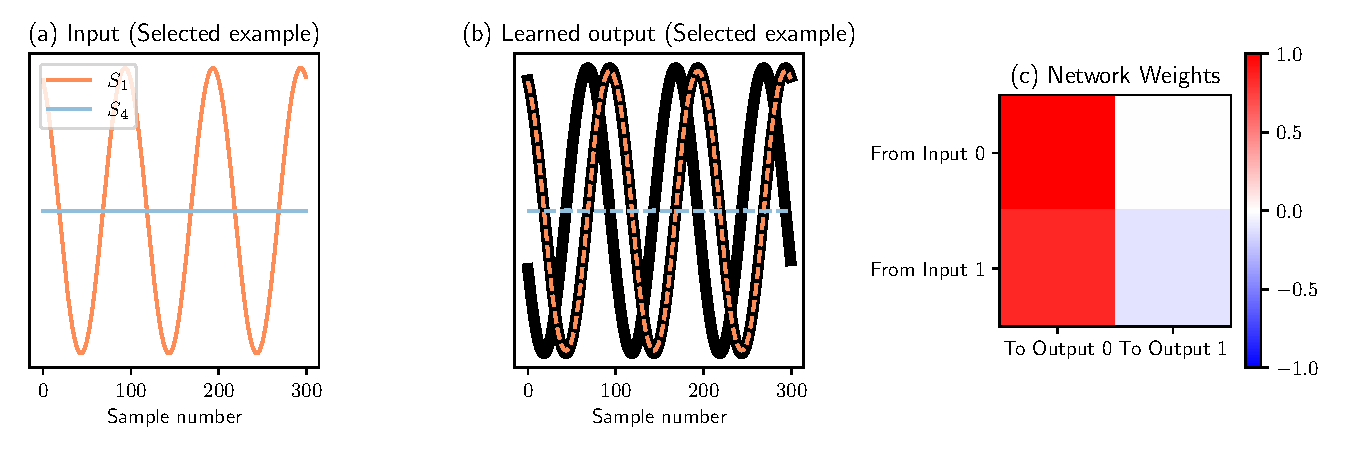
\includegraphics[width=1\linewidth]{neural_network_2}
  	\caption{Similar to figure \ref{fig:neuralnetwork0} but for input signal $S_4$ applied to input $I_2$.}
  	\label{fig:neuralnetwork2}
\end{figure*} 

In conclusion, figures \ref{fig:neuralnetwork0}-\ref{fig:neuralnetwork2} demonstrate that the task presented by \citet{Annand2020} can be considered as consisting of two independent subtasks. Controlling the $Y$-position of the stylus on does not dependent on (the accuracy of) controlling the $X$-position. 

\section{Reanalysis of empirical data}

The previous section shows that, in principle, the task can considered as consisting of two independent subtasks. However, this does not necessarily imply that participants did solve the task in this way. To assess whether participants deconstructed the task into two components, we reanalysed the data presented in figures 5 and 6 in the paper by \citet{Annand2020}.

In figure 5, \citet{Annand2020} plot the $X$ and $Y$ position of the stylus, as controlled by a participant, together with the desired target positions. They plot these data for trial 1, 5, 15 and 20. Using the Open Source software Engauge Digitizer, we digitized the data in these graphs, sampling the curves at a rate of 10 Hz. For each trial for which data was provided we calculated the error signals,
%
\begin{eqnarray}
\Delta x_t = p_{x,t} - t_{x,t}\\
\Delta y_t = p_{y,t} - t_{y,t}
\end{eqnarray}
%
with $p_{x,t}$ ($p_{x,t}$) the position of the stylus as controlled by the participant at time $t$. Conversely, $t_{x,t}$ and $ t_{y,t}$ denote the position of the target on the screen.

To assess the amount of coupling between the $X$ and $Y$ position of the stylus as a function of trial number, we analyze the error signals $\Delta x_i$ and $\Delta y_i$. The justification for is the demonstration (previous section) that perfect performance can not be interpreted as evidence for coupling between limbs or participants of a dyad. Alternatively, the errors could be be coupled. To assess this, we calculated the short term, normalized, cross correlation between $\Delta x_i$ and $\Delta y_i$,
%
\begin{equation}
k_t = \max_t \frac{| \Delta x [t,t+3] \star \Delta y [t,t+3] |}{\sqrt{(\Delta x [t,t+3]  \star \Delta x [t,t+3] )^2 \times (\Delta y [t,t+3]  \star \Delta y [t,t+3] )^2} }
\label{eq:cross}
\end{equation}
%
Equation \ref{eq:cross} gives the normalized cross correlation (i.e., ranges -1 to +1) for a 3 second windowed interval of the error signals. Next, we calculated the average short term, normalized cross correlation across the full signals from $t=0$ to $t=T$,
%
\begin{equation}
\bar{k} = \frac{1}{T} \sum_0^T k_t
\end{equation}.

This averaged value, $\bar{k}$, gives the average cross correlation between the error signals $\Delta x_i$ and $\Delta y_i$, considered in 3 second intervals, across the full signals. As such, it presents a measure of how much the error $\Delta x_i$ depends on the error $\Delta Y_i$ over the complete duration of the trial. 

Values for $\bar{k}$ larger than zero indicate that participants tried to correct any deviation between $p_{x,i}$ and $t_{x_i}$ by introducing errors in the $Y$-direction, or vice versa. In other words, $\bar{k}$ provides an insight in \textit{how} the participants attempted to reduce errors.

In figure \ref{fig:reanalysis}, we plot $\bar{k}$  as a function of trial number. We also compare this with average RMSE values for each trial. The RMSE is used by \citet{Annand2020} to quantify performance. As can be seen, as performance increases (measured by RMSE), the error cross correlation $\bar{k}$ decreases. This suggests that participants increased performance by \textit{decoupling} their limbs such that errors the $X$-direction did not result in errors in the $Y$-direction. Note also that the short term correlation between errors is substantial: it varies between about 0.8 and 0.5.

\begin{figure}
	\centering
	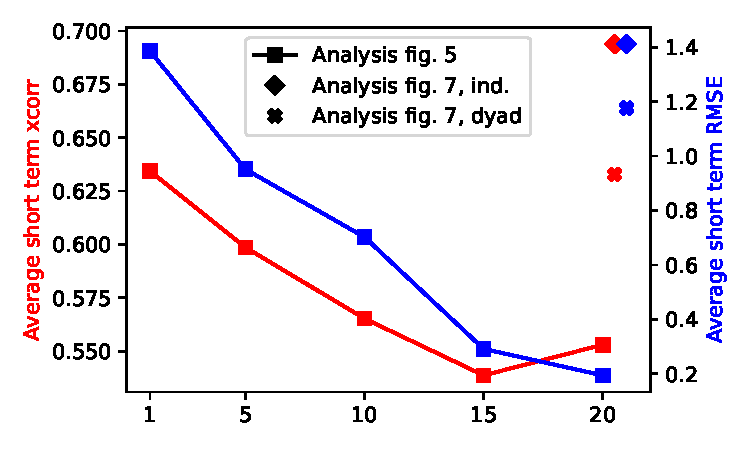
\includegraphics[width=1\linewidth]{reanalysis}
	\caption{Average short term cross-correlation for the error signals derived from fig. 5 in \citet{Annand2020} as function of trial number. The graph also shows the RMSE. In addition, the plot shows the data points derived from fig. 7 in \citet{Annand2020} for an individual and a dyad whose performance did not increase with training.}
	\label{fig:reanalysis}
\end{figure}

\citet{Annand2020} noted that a number of dyads and individuals did not attain good performance, even after 20 trials. They show the behavior on a final trial for one such individual and one such dyad in figure 7. We analyzed these data in the same manner as the data in their figure 5 and added the result to the graph in figure \ref{fig:reanalysis}. This shows that this individual and dyad performed poorly (high RMSE) as they failed to decouple the control for the $X$ and the $Y$ directions (high $\bar{k}$).

In conclusion, a reanalysis of the data presented in the paper by \citet{Annand2020} shows that an increase in performance depended on a decrease in coupling between the two limbs (or the individuals in the dyads). Our computational analysis has already shown that trying to compensate for errors in one direction by adjusting the other direction is not required for optimal performance. This reanalysis shows that such behavior also decreased performance.

\section{Coupling is unlikely to increase performance}

So far, we have shown that the task of \citet{Annand2020} does not require coupling between limbs. Moreover, we have shown that their participants increased performance while decoupling the limbs. However, this does not exclude that coupling could be used to increase task performance. In this section, we address this question.

As said before, \citet{Annand2020} do not formalize the concept of coupling. However, as we have shown that perfect performance does not require coupling, we propose that coupling might be detect by analysis of the errors. Indeed, this assumption formed the basis of our previous analysis.

Here, we present a Monte Carlo simulation to assess whether the performance, as quantified by the RMSE, could be increased by coupling. Because \citet{Annand2020} do not formalize coupling, we propose the following, the degree of coupling between the limbs is a function of the correlation and time shift between the error signals $\Delta x_i$ and $\Delta y_i$. In other words, we propose that coupling between the limbs implies,

\begin{equation}
\mbox{Need better equation here}
\label{eq:coupling}
\end{equation}
%

In our Monte Carlo analysis, we generated error signals $\Delta x_t$ and $\Delta y_t$. These were obtained by sampling from a normal distribution ($\mu = 0, \rho=1$).  The signals were smoothed using a box window (7 samples) to obtain signals whose temporal auto-correlation matched those of the empirical error signals as reported by \citet{Annand2020}.

We varied the amount of coupling. In particular, we varied $0 \leq r \leq 1$. Moreover, we considered two time shifts  $\delta t =$ 0, 0.1, 0.5 and 1.5 seconds. It should be noted that the lag between the error signals depicted in figure 5 is about 1.5 seconds.

Next, we plotted the average RMSE as a function of correlation $r$ and time shift  $\delta t$ (figure \ref{fig:correlation}). This graphs shows that, in the absence of a time shift ( $\delta t = 0$), increasing the correlation $r$ does reduce the error somewhat (by maximally 10 percent for $r=1$). However, introducing a time shift cancels this effect. Indeed, for a time shift of 0.5 seconds, not benefit of coupling (high correlation) was observed.


\begin{figure}
	\centering
	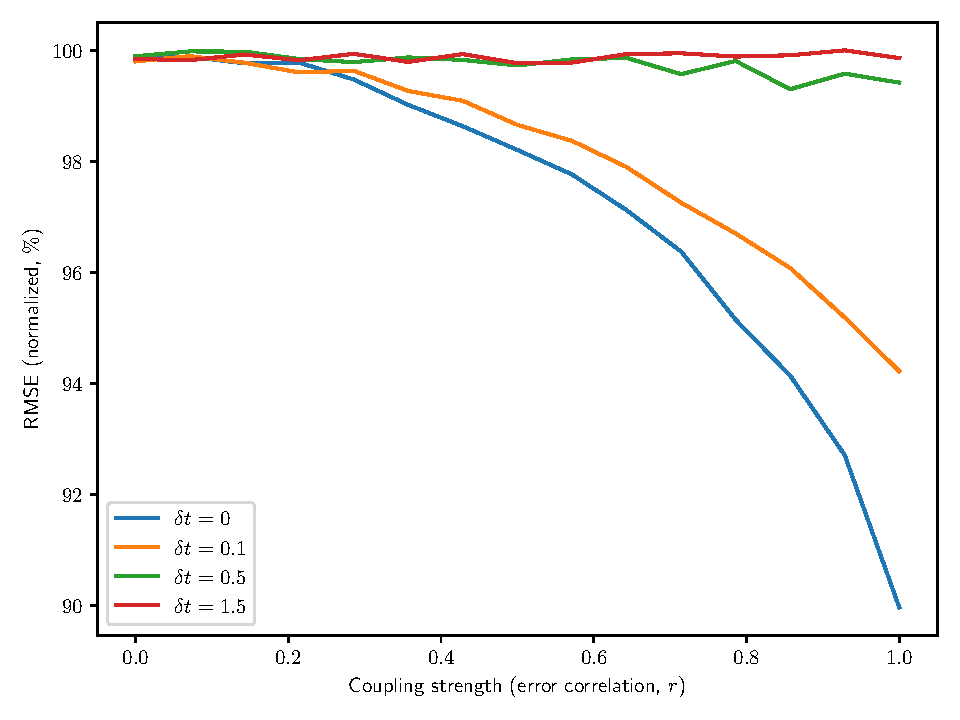
\includegraphics[width=1\linewidth]{correlation}
	\caption{asdasda}
	\label{fig:correlation}
\end{figure}

From figure \ref{fig:correlation}, we conclude that, in principle, individual participants could have derived some benefit from rigorously coupling their limbs. However, this would require ensuring that they are coupled both with a minimal time lag and high degree of rigidity. 

\bibliographystyle{plainnat}
\bibliography{refs}


\end{document}
